\documentclass[preprint, hmargin=1in, vmargin=1in]{aastex62}
%%%%%%begin preamble
%\usepackage[hmargin=1in, vmargin=1in]{geometry} % Margins
\usepackage{hyperref}
\usepackage{url}
\usepackage{natbib}
\setlength{\bibsep}{0pt plus 0.3ex}
\usepackage{graphicx}
\usepackage{amsmath}
\usepackage{amsfonts}
\usepackage{amssymb}
%\usepackage{import}
\usepackage{wrapfig}
\usepackage{changepage}
\usepackage{lipsum}

\usepackage{color}
\hypersetup{
  colorlinks   = true,
  %citecolor    = blue
  citecolor    = gray
  % gray is not being found!?!
  % gray is found if pdfpages is used... crap.
  %citecolor    = grey
  %citecolor    = Gray
}

%% headers
\usepackage{fancyhdr}
\pagestyle{fancy}
\fancyhf{} % sets both header and footer to nothing
\lhead{Evan Anders -- Research Statement}
\rhead{CITA Postdoctoral Fellowship}
\cfoot{\footnotesize{\thepage}}
%\pagestyle{empty}
%\pagenumbering{gobble}
%\renewcommand*{\thefootnote}{\fnsymbol{footnote}}

\renewcommand{\vec}{\ensuremath{\boldsymbol}}
\newcommand{\dedalus}{\href{http://dedalus-project.org}{Dedalus}}
\newcommand{\del}{\ensuremath{\vec{\nabla}}}
\newcommand{\scrS}{\ensuremath{\mathcal{S}}}

\newcommand{\prf}{Physical Review Fluids}

%\newcommand{\nosection}[1]{%
%  \refstepcounter{section}%
%  \addcontentsline{toc}{section}{\protect\numberline{\thesection}#1}%
%  \markright{#1}}
%\newcommand{\nosubsection}[1]{%
%  \refstepcounter{subsection}%
%  \addcontentsline{toc}{subsection}{\protect\numberline{\thesubsection}#1}%
%  \markright{#1}}

%\usepackage{atbegshi}
%%%%%%end preamble


\begin{document}
\maketitle
\vspace{-88pt}
\section*{\textbf{Motivation}}
\thispagestyle{fancy}
Main sequence stars with masses similar to the Sun have envelopes of vigorous convection.
These convecting regions are highly stratified (14 density scale heights in the Sun), and the convective motions generate sound waves which refract due to stratification as they propagate in the stellar interior.
Helioseismology and asteroseismology measure the surface signatures of these waves to examine the interior of the Sun and other stars.
These measurements have enabled the precise determination of mass and radius of many stars, and have revealed the interior structure and mean flows, like differential rotation, inside the Sun \citep{huber&all2019, christensen-dalsgaard2002}.


Interpretation of asteroseismic data relies on one-dimensional (1D) stellar structure models. 
State-of-the-art codes like MESA \citep{paxton&all2011} which generate 1D stellar structure profiles have known deficiencies \citep{buldgen2019}, including their use of convective parameterizations like mixing length theory \citep[MLT,][]{bohm-vitense1958}.
MLT assumes that stellar convection zones generate flows with length scales proportional to the atmospheric scale height throughout their whole radial extent.
MLT thus predicts that small convection cells driven near the stellar photosphere should overlie large-scale ``giant cells'' driven in the deep convection zone.
Giant cells have not been detected in helioseismic observations or direct measurements of flows at the Sun's photosphere \citep{hanasoge&all2015, hathaway&all2015}.
The absence of giant cells is called the ``Solar Convective Conundrum'' and demonstrates that our fundamental understanding of stellar convection is flawed.
We must come to a new understanding of stellar convection by solving the Convective Conundrum, and in doing so improving stellar structure models and asteroseismic observations.

In my research, I use the Dedalus code \citep{burns&all2019} to create simulations of stellar convection to help solve the Convective Conundrum.
Parameterizations like MLT generally neglect rotation and magnetism, but asteroseismic measurements are affected by the morphology of rotational and magnetic profiles \citep{benomar&all2018, santos&all2018} and these effects may be able to suppress giant cells \citep{featherstone&hindman2016}.
As a modeling community, we must therefore work to understand how rotation and magnetism affect stellar structure and convection.
As a CITA fellow, I will study three targeted investigations to discover how rotation and magnetism affect flows in stellar envelope convection using simulations which span from the smallest to largest scales present in stars.

\section*{\textbf{Numerical Studies of Stellar Convection Across All Scales}}
\paragraph{The Entropy Rain Hypothesis}
Convection which occurs in the presence of atmospheric density stratification exhibits asymmetrical upflows and downflows.
Upwellings are slow, weak, and wide while downflows are intense, fast, and narrow.
The ``entropy rain'' hypothesis \citep[][]{spruit1997} posits that downflows alone may be sufficiently powerful in stellar envelope convection to transport the stellar luminosity.
Upflows with negligible energy transport would exist alongside these downflows mostly to conserve mass.
This hypothesis, and the nontraditional dynamical form of convection it suggests, could explain the absence of giant cells in observations.
Recent simulations of envelope convection suggest that surface-driven downflows can transport most of the stellar luminosity \citep{kapyla&all2017}, and a modified MLT with entropy rain was recently derived by \citet{brandenburg2016}.
A schematic of the entropy rain picture is shown in Fig.~\ref{fig:tri_panel}a.
All theoretical work regarding the entropy rain hypothesis has thusfar been purely hydrodynamical, so we do not know how rotation and magnetism affect the entropy rain picture.


\paragraph{Convection at the Smallest Scales: Individual Downflows} 
The entropy rain hypothesis suggests that we should study the nonlocal effects of stellar downflows more carefully.
These downflows may turbulently break up into distinct pieces as they fall and these individual pieces can be modeled as ``thermals.''
Thermals are regions of cold fluid which accelerate due to buoyancy forces and shape themselves into vortex rings; an evolved turbulent thermal is visualized in Fig. \ref{fig:tri_panel}b.
Thermals are also observed and studied in the Earth's atmosphere \citep{lecoanet&jeevanjee2019}.
In \citet{andersLB2019}, I studied how an atmospheric density stratification affects the size of thermals as they propagate.
I found that thermals compress less than a simple stratification-based estimate would anticipate \citep{brandenburg2016}.
I surprisingly found that thermal-like downflows could carry the Sun's luminosity, which agrees with the entropy rain hypothesis.

\begin{figure*}[t]
    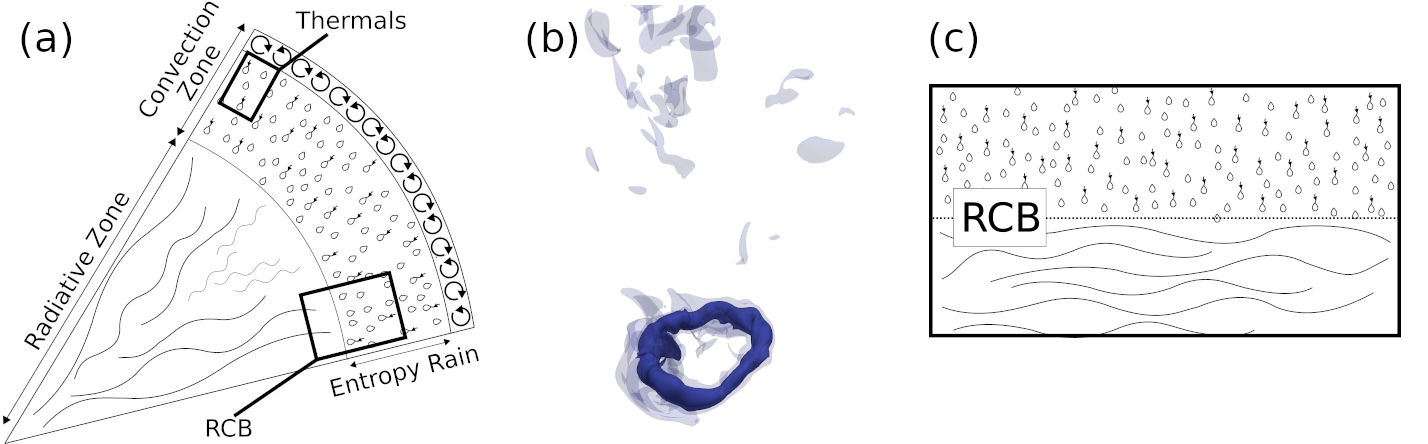
\includegraphics[width=\textwidth]{./figs/tri_panel.png}
    \caption{ (a) A schematic of the interior of solar-type stars under the entropy rain hypothesis, where cold droplets of fluid carry the stellar luminosity below a small traditional convective surface layer.
	The scope of the first two experiments described in this section are boxed and labeled (``Thermals'' and ``RCB'').
	(b) A 3D visualization of entropy perturbations within the downward-propagating reference frame of a turbulent thermal, which may be the dynamical form of entropy rain.
	(c) A schematic of the radiative-convective boundary (RCB), where downflows impinge upon a stable layer and excite gravity waves within that layer.
	\label{fig:tri_panel} }
\end{figure*}

As a CITA fellow, I will build upon my thesis study of thermals-as-downflows \citep{andersLB2019} by learning how rotation and magnetism affect the ability of downflows to transit a stellar convection zone.
These physical complications could have filtering effects on downflows, preventing their successful propagation through the stellar convection zone in certain regimes.
I will determine whether strong magnetic fields or rapid global rotation can ``evaporate'' entropy rain.
Constraining the regimes in which these realistic effects prevent downflows from crossing the stellar convection zone is crucial to determining the validity of the entropy rain hypothesis.

\paragraph{Convection at the Mesoscale: Interactions at the Radiative-Convective Boundary}
In solar-type stars, a radiative-convective boundary (RCB) sits at the base of the turbulent convection zone; beneath the RCB, radiation effectively carries the stellar luminosity in a stably stratified radiative zone.
The solar RCB coincides with a region of intense radial velocity shear called the tachocline, and it is thought that tachocline shear interactions are a crucial driver of the Sun's magnetic dynamo.
In order to better understand deep convection and to figure out how stars drive their dynamos and differential rotation profiles, we must constrain the pumping of angular momentum and magnetism by downflows into the RCB.

As a CITA fellow, I will study how an ensemble of downflows interacts with a solar-like RCB in the presence of rotation and magnetism to constrain the importance of the RCB in establishing the stellar rotation profile and magnetic dynamo.
I will simulate time-evolving mesoscale convection with unstable convection zones above stable radiative interiors, as depicted in Fig.~\ref{fig:tri_panel}c.
This study naturally extends my PhD studies of stratified convection \citep{anders&brown2017, anders&all2019} in setups similar to those in \citet{kapyla&all2017} where downflows were found to be dominant. 
%These simulations will naturally build upon my proposed thermals-as-downflows simulations, because I will only study RCB interactions in the regimes where downflows are not evaporated by rotation and magnetism.
These simulations will determine if the RCB and tachocline are primary drivers of stellar dynamos by constraining the efficiency of magnetic pumping into the RCB.
In addition to helping determine where stellar dynamos are driven, these studies will help determine the stellar rotation rates and luminosities in which downflows can effectively establish solar-like differential rotation profiles and tachoclines through RCB interactions, building on the recent work of \citet{wood&brummell2018}.

\paragraph{Global Scale Convection: Dynamics in Relaxed Atmospheres}
Some modern studies seek to remove the need for parameterizations like MLT by coupling 1D stellar structure models with fully convective, three-dimensional (3D) global simulations.
Recently, to great success, \citet{jorgensen&weiss2019} coupled 1D models to previously-computed 3D spherical shell simulations of convection in thin, near-surface layers.
Such a coupling has not yet been performed for deep convection, where most disagreements between simulations and observations occur \citep[the Convective Conundrum,][]{hanasoge&all2015}.
In near-surface shells, the convective overturn timescale is very similar to the local Kelvin-Helmholtz (KH) timescale of atmospheric equilibration.
However, in deep, turbulent convection, many overturn timescales pass during one KH timescale; simulations with deep convection therefore must evolve through a long and scientifically-uninteresting thermal rundown before convective statistics can be sampled.
Creating simulations of deep convection for arbitrary stars which can be coupled with 1D models is therefore too computationally expensive using traditional timestepping techniques.
In \citet{anders&all2018}, I found a mechanism for fast-forwarding through the KH timescale in a simple convective system.
I verified that my fast-forwarding procedure produced the same results as standard timestepping techniques to within 1\%.
This accuracy was achieved using an order of magnitude fewer cpu-hours than traditional techniques.


\begin{wrapfigure}{r}{0.3\textwidth}
	\begin{center}
	\vspace{-16pt}
    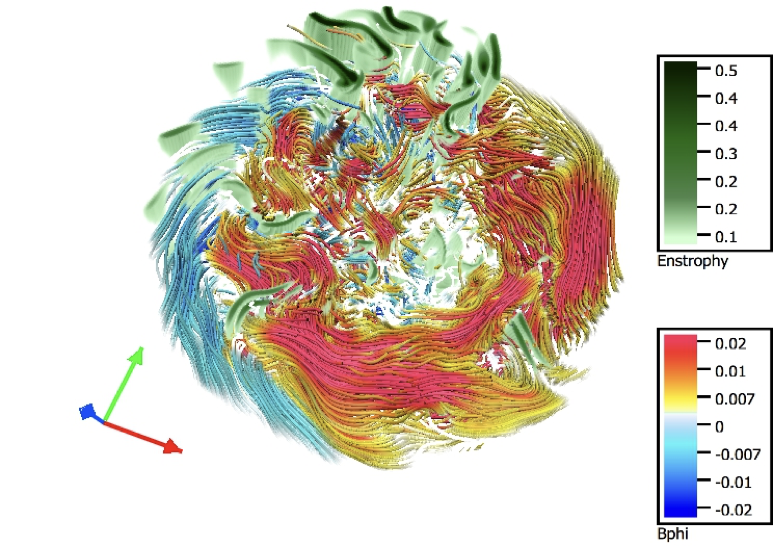
\includegraphics[width=0.28\textwidth]{./figs/mdwarf.png}
	\vspace{-16pt}
	\end{center}
    \caption{A volume rendering of a global dynamo simulation in Dedalus.
	Enstrophy, or the magnitude of vorticity, is shown in green.
	Red and blue lines denote the magnitude and direction of azimuthal magnetic field.
	\label{fig:mdwarf} }
	\vspace{-16pt}
\end{wrapfigure}
As a CITA fellow, I will extend my PhD accelerated evolution method \citep{anders&all2018} by creating and validating a generalized public module which rapidly equilibrates mean thermodynamic profiles and flows in global simulations of deep convection.
I will use Dedalus, which can accurately simulate deep convective motions in global domains that include the origin at $r = 0$ \citep[as visualized in Fig.~\ref{fig:mdwarf}, and tested in][]{lecoanet&all2019}, to test the accuracy of this tool.
This module will effectively take KH-size timesteps by reading in statistical measures from unequilibrated convection and solving for an equilibrated mean state.
Researchers simulating global convection using arbitrary codes will be able to use this module to rapidly equilibrate simulations with state-of-the-art turbulent dynamics.
Statistics of deep convection can be sampled from these converged states and coupled with 1D models in the same manner as \citet{jorgensen&weiss2019} coupled simulations of surface convection.
In addition to creating and validating this tool, I will employ it in my research to study RCB interactions in global simulations to learn how spherical effects (e.g., mean flows and geometry) affect pumping into the RCB.
Furthermore, \citet{featherstone&hindman2016} found that rapid rotation could suppress giant cells in global simulations in some regimes.
I will determine if this suppression of giant cells occurs in regimes where my thermals-as-downflows studies determined that entropy rain does not evaporate.
If these regimes align, it is likely that rotational effects and nonlocal transport of energy by entropy rain together provide a partial solution to the Convective Conundrum.


\section*{\textbf{Collaborative Studies at CITA}}
CITA is the ideal location to carry out this proposed research due to the cross-disciplinary collaborations available with astrophysicists spanning broad research interests.
This work is crucial to understanding the life cycles and death of stars similar to the Sun, and thus fits naturally with CITA's research goals.
I look forward to collaborating with the many experts in astrophysical fluid dynamics at CITA like Prof.~Norman Murray, as well as future and current CITA fellows such as Drs.~Tricco, Yalinewich, and Zanazzi.
In addition to the projects proposed here, I am excited about the opportunity to use Dedalus' flexibility to pursue research questions that I have yet to consider with members of both the Black Holes, Neutron Stars, \& White Dwarfs group as well as the Planets \& Planetary Systems group.
I look forward to the opportunity to create cross-disciplinary collaborations and to carry on the CITA's excellent research tradition while making lasting contributions towards solving the Convective Conundrum.

\bibliographystyle{yahapj}
\bibliography{biblio}
\end{document}
